% Options for packages loaded elsewhere
\PassOptionsToPackage{unicode}{hyperref}
\PassOptionsToPackage{hyphens}{url}
%
\documentclass[
]{article}
\usepackage{lmodern}
\usepackage{amssymb,amsmath}
\usepackage{ifxetex,ifluatex}
\ifnum 0\ifxetex 1\fi\ifluatex 1\fi=0 % if pdftex
  \usepackage[T1]{fontenc}
  \usepackage[utf8]{inputenc}
  \usepackage{textcomp} % provide euro and other symbols
\else % if luatex or xetex
  \usepackage{unicode-math}
  \defaultfontfeatures{Scale=MatchLowercase}
  \defaultfontfeatures[\rmfamily]{Ligatures=TeX,Scale=1}
\fi
% Use upquote if available, for straight quotes in verbatim environments
\IfFileExists{upquote.sty}{\usepackage{upquote}}{}
\IfFileExists{microtype.sty}{% use microtype if available
  \usepackage[]{microtype}
  \UseMicrotypeSet[protrusion]{basicmath} % disable protrusion for tt fonts
}{}
\makeatletter
\@ifundefined{KOMAClassName}{% if non-KOMA class
  \IfFileExists{parskip.sty}{%
    \usepackage{parskip}
  }{% else
    \setlength{\parindent}{0pt}
    \setlength{\parskip}{6pt plus 2pt minus 1pt}}
}{% if KOMA class
  \KOMAoptions{parskip=half}}
\makeatother
\usepackage{xcolor}
\IfFileExists{xurl.sty}{\usepackage{xurl}}{} % add URL line breaks if available
\IfFileExists{bookmark.sty}{\usepackage{bookmark}}{\usepackage{hyperref}}
\hypersetup{
  pdftitle={Lesson 7 Companion},
  hidelinks,
  pdfcreator={LaTeX via pandoc}}
\urlstyle{same} % disable monospaced font for URLs
\usepackage[margin=1in]{geometry}
\usepackage{color}
\usepackage{fancyvrb}
\newcommand{\VerbBar}{|}
\newcommand{\VERB}{\Verb[commandchars=\\\{\}]}
\DefineVerbatimEnvironment{Highlighting}{Verbatim}{commandchars=\\\{\}}
% Add ',fontsize=\small' for more characters per line
\usepackage{framed}
\definecolor{shadecolor}{RGB}{248,248,248}
\newenvironment{Shaded}{\begin{snugshade}}{\end{snugshade}}
\newcommand{\AlertTok}[1]{\textcolor[rgb]{0.94,0.16,0.16}{#1}}
\newcommand{\AnnotationTok}[1]{\textcolor[rgb]{0.56,0.35,0.01}{\textbf{\textit{#1}}}}
\newcommand{\AttributeTok}[1]{\textcolor[rgb]{0.77,0.63,0.00}{#1}}
\newcommand{\BaseNTok}[1]{\textcolor[rgb]{0.00,0.00,0.81}{#1}}
\newcommand{\BuiltInTok}[1]{#1}
\newcommand{\CharTok}[1]{\textcolor[rgb]{0.31,0.60,0.02}{#1}}
\newcommand{\CommentTok}[1]{\textcolor[rgb]{0.56,0.35,0.01}{\textit{#1}}}
\newcommand{\CommentVarTok}[1]{\textcolor[rgb]{0.56,0.35,0.01}{\textbf{\textit{#1}}}}
\newcommand{\ConstantTok}[1]{\textcolor[rgb]{0.00,0.00,0.00}{#1}}
\newcommand{\ControlFlowTok}[1]{\textcolor[rgb]{0.13,0.29,0.53}{\textbf{#1}}}
\newcommand{\DataTypeTok}[1]{\textcolor[rgb]{0.13,0.29,0.53}{#1}}
\newcommand{\DecValTok}[1]{\textcolor[rgb]{0.00,0.00,0.81}{#1}}
\newcommand{\DocumentationTok}[1]{\textcolor[rgb]{0.56,0.35,0.01}{\textbf{\textit{#1}}}}
\newcommand{\ErrorTok}[1]{\textcolor[rgb]{0.64,0.00,0.00}{\textbf{#1}}}
\newcommand{\ExtensionTok}[1]{#1}
\newcommand{\FloatTok}[1]{\textcolor[rgb]{0.00,0.00,0.81}{#1}}
\newcommand{\FunctionTok}[1]{\textcolor[rgb]{0.00,0.00,0.00}{#1}}
\newcommand{\ImportTok}[1]{#1}
\newcommand{\InformationTok}[1]{\textcolor[rgb]{0.56,0.35,0.01}{\textbf{\textit{#1}}}}
\newcommand{\KeywordTok}[1]{\textcolor[rgb]{0.13,0.29,0.53}{\textbf{#1}}}
\newcommand{\NormalTok}[1]{#1}
\newcommand{\OperatorTok}[1]{\textcolor[rgb]{0.81,0.36,0.00}{\textbf{#1}}}
\newcommand{\OtherTok}[1]{\textcolor[rgb]{0.56,0.35,0.01}{#1}}
\newcommand{\PreprocessorTok}[1]{\textcolor[rgb]{0.56,0.35,0.01}{\textit{#1}}}
\newcommand{\RegionMarkerTok}[1]{#1}
\newcommand{\SpecialCharTok}[1]{\textcolor[rgb]{0.00,0.00,0.00}{#1}}
\newcommand{\SpecialStringTok}[1]{\textcolor[rgb]{0.31,0.60,0.02}{#1}}
\newcommand{\StringTok}[1]{\textcolor[rgb]{0.31,0.60,0.02}{#1}}
\newcommand{\VariableTok}[1]{\textcolor[rgb]{0.00,0.00,0.00}{#1}}
\newcommand{\VerbatimStringTok}[1]{\textcolor[rgb]{0.31,0.60,0.02}{#1}}
\newcommand{\WarningTok}[1]{\textcolor[rgb]{0.56,0.35,0.01}{\textbf{\textit{#1}}}}
\usepackage{graphicx,grffile}
\makeatletter
\def\maxwidth{\ifdim\Gin@nat@width>\linewidth\linewidth\else\Gin@nat@width\fi}
\def\maxheight{\ifdim\Gin@nat@height>\textheight\textheight\else\Gin@nat@height\fi}
\makeatother
% Scale images if necessary, so that they will not overflow the page
% margins by default, and it is still possible to overwrite the defaults
% using explicit options in \includegraphics[width, height, ...]{}
\setkeys{Gin}{width=\maxwidth,height=\maxheight,keepaspectratio}
% Set default figure placement to htbp
\makeatletter
\def\fps@figure{htbp}
\makeatother
\setlength{\emergencystretch}{3em} % prevent overfull lines
\providecommand{\tightlist}{%
  \setlength{\itemsep}{0pt}\setlength{\parskip}{0pt}}
\setcounter{secnumdepth}{-\maxdimen} % remove section numbering

\title{Lesson 7 Companion}
\author{}
\date{\vspace{-2.5em}}

\begin{document}
\maketitle

\hypertarget{research-question}{%
\subsubsection{Research question:}\label{research-question}}

For this example I'm going to use the data available on the book's
website for the ``Time Estimate'' problem. It doesn't match the exact
data in the textbook (for some reason) but it'll work for this example.

Remember the research question is whether or not people can accurately
estimate the length of a short song snippet. The parameter of interest
is the population average length estimate (\(\mu\)), the statistic is
the sample average length estimate (\(\bar{x}\)), and the hypothesis are
as follows:

\(H_{0}: \mu = 10\)

\(H_{a}: \10 \neq 10\)

\hypertarget{simulation-based-approach}{%
\subsubsection{Simulation-based
Approach}\label{simulation-based-approach}}

I always tell my students that, at the end of this discussion, you feel
like we've done something sketchy then you probably grasp the concepts.
Rest assured that, however sketchy it may feel, what we are about to do
is grounded in solid statistics.

\begin{Shaded}
\begin{Highlighting}[]
\KeywordTok{library}\NormalTok{(tidyverse)}
\KeywordTok{library}\NormalTok{(patchwork) }\CommentTok{#Install this if you want to use it}

\NormalTok{estimates =}\StringTok{ }\KeywordTok{read_table2}\NormalTok{(}\StringTok{"http://www.isi-stats.com/isi/data/chap3/TimeEstimate.txt"}\NormalTok{)}

\KeywordTok{head}\NormalTok{(estimates)}
\end{Highlighting}
\end{Shaded}

\begin{verbatim}
## # A tibble: 6 x 1
##    Time
##   <dbl>
## 1     6
## 2     7
## 3     7
## 4     9
## 5     9
## 6     9
\end{verbatim}

\begin{Shaded}
\begin{Highlighting}[]
\NormalTok{sample_stat =}\StringTok{ }\KeywordTok{mean}\NormalTok{(estimates}\OperatorTok{$}\NormalTok{Time)}

\NormalTok{new_population =}\StringTok{ }\KeywordTok{do.call}\NormalTok{(}\StringTok{"rbind"}\NormalTok{, }\KeywordTok{replicate}\NormalTok{(}\DecValTok{10}\NormalTok{, estimates, }\DataTypeTok{simplify =} \OtherTok{FALSE}\NormalTok{))}

\NormalTok{null_mean =}\StringTok{ }\DecValTok{10}

\NormalTok{new_population =}\StringTok{ }\NormalTok{new_population }\OperatorTok{-}\StringTok{ }\KeywordTok{abs}\NormalTok{(}\KeywordTok{mean}\NormalTok{(new_population}\OperatorTok{$}\NormalTok{Time) }\OperatorTok{-}\StringTok{ }\DecValTok{10}\NormalTok{)}

\NormalTok{p1 <-}\StringTok{ }\NormalTok{estimates }\OperatorTok
\StringTok{  }\KeywordTok{ggplot}\NormalTok{(}\KeywordTok{aes}\NormalTok{(}\DataTypeTok{x =}\NormalTok{ Time)) }\OperatorTok{+}
\StringTok{  }\KeywordTok{labs}\NormalTok{(}\DataTypeTok{x =} \StringTok{"Time"}\NormalTok{, }\DataTypeTok{y =} \StringTok{"Count"}\NormalTok{, }\DataTypeTok{title =} \StringTok{"Distribution of Original Sample"}\NormalTok{) }\OperatorTok{+}
\StringTok{  }\KeywordTok{geom_histogram}\NormalTok{()}

\NormalTok{p2 <-}\StringTok{ }\NormalTok{new_population }\OperatorTok
\StringTok{  }\KeywordTok{ggplot}\NormalTok{(}\KeywordTok{aes}\NormalTok{(}\DataTypeTok{x =}\NormalTok{ Time)) }\OperatorTok{+}
\StringTok{  }\KeywordTok{labs}\NormalTok{(}\DataTypeTok{x =} \StringTok{"Time"}\NormalTok{, }\DataTypeTok{y =} \StringTok{"Count"}\NormalTok{, }\DataTypeTok{title =} \StringTok{"Distribution of New Population"}\NormalTok{) }\OperatorTok{+}
\StringTok{  }\KeywordTok{geom_histogram}\NormalTok{()}

\NormalTok{p1 }\OperatorTok{+}\StringTok{ }\NormalTok{p2}
\end{Highlighting}
\end{Shaded}

\begin{center}\includegraphics[width=0.7\linewidth,height=0.7\textheight]{Lesson-7-Companion_files/figure-latex/unnamed-chunk-1-1} \end{center}

Let's take this part-by-part to help explain what is going in. After
loading the libraries we will need, we load the dataset from the book's
website. I can check to ensure that it was loaded correctly (and get the
column title) using the head command. My next step is to start building
my new population by copying the estimates dataframe ten times. The
\textbf{do.call} function performs whatever function is listed (in this
case \textbf{r}ow \textbf{bind}) given the arguments that are listed
next. Here we are binding these ten replicates for our empirical
datasets into a single dataframe.

The next step is to shift the mean of our new population. Recall that
the purpose of building this new population is to have a population to
sample from to build the null distribution. Of course you recall that,
when you are building the null distribution, you assume the truth of the
null hypothesis. In this problem our null hypothesis is that the average
estimate will be 10 seconds. Therefore we need to build a population
where the mean is 10 seconds. We can do this by finding the absolute
value of the difference between the real mean of the new population and
our null mean (\textbf{abs(mean(new\_population\$Time) - 10)}) and
subtracting that from every element in the \textbf{new\_population}
dataframe.

So now that we have this new population with a mean of 10
seconds\ldots{} let's reflect on how this could possibly be an
acceptable method. Consider that what we are really looking for when
building our null distribution is an idea of how spread out we can
expect the results to be. When we built the null distribution using coin
flips for the Doris and Buzz problem we were trying to see how spread
out the simulated results were. Ultimately, it answered the question:
how likely would it be to see 15 heads by chance alone? This is a
question of the variation of our results.

Take a look at the two plots here and consider, even when we have
shifted our mean, are we capturing the spread of our empirical sample?
Of course we are! Since we merely replicated the sample ten times
(ignoring the y-axis) our histograms look exactly the same. Now we can
get to the actual work of building our simulated null hypothesis.

\begin{Shaded}
\begin{Highlighting}[]
\NormalTok{replications_dataframe =}\StringTok{ }\OtherTok{NULL}

\NormalTok{num_reps =}\StringTok{ }\DecValTok{1000}

\NormalTok{sample_size =}\StringTok{ }\DecValTok{25} \CommentTok{#Original sample size}

\ControlFlowTok{for}\NormalTok{ (i }\ControlFlowTok{in} \DecValTok{1}\OperatorTok{:}\NormalTok{num_reps)\{}
  
\NormalTok{  trial =}\StringTok{ }\KeywordTok{sample}\NormalTok{(new_population}\OperatorTok{$}\NormalTok{Time, }
                 \DataTypeTok{size =}\NormalTok{ sample_size, }
                 \DataTypeTok{replace =} \OtherTok{FALSE}\NormalTok{)}
  
\NormalTok{  trial_stat =}\StringTok{ }\KeywordTok{mean}\NormalTok{(trial)}
  
\NormalTok{  replications_dataframe =}\StringTok{ }\KeywordTok{rbind}\NormalTok{(replications_dataframe, }\KeywordTok{data.frame}\NormalTok{(trial_stat))}
  
\NormalTok{\}}

\CommentTok{#Calculate how far away from the null mean}
\CommentTok{# our sample mean was.}
\NormalTok{dist_from_null =}\StringTok{ }\KeywordTok{abs}\NormalTok{(sample_stat }\OperatorTok{-}\StringTok{ }\NormalTok{null_mean)}

\CommentTok{#Value above the null mean}
\NormalTok{above =}\StringTok{ }\NormalTok{null_mean }\OperatorTok{+}\StringTok{ }\NormalTok{dist_from_null}

\CommentTok{#Value below the null mean}
\NormalTok{below =}\StringTok{ }\NormalTok{null_mean }\OperatorTok{-}\StringTok{ }\NormalTok{dist_from_null}

\NormalTok{replications_dataframe }\OperatorTok
\StringTok{  }\KeywordTok{ggplot}\NormalTok{(}\KeywordTok{aes}\NormalTok{(}\DataTypeTok{x =}\NormalTok{ trial_stat)) }\OperatorTok{+}
\StringTok{  }\KeywordTok{geom_histogram}\NormalTok{() }\OperatorTok{+}
\StringTok{  }\KeywordTok{labs}\NormalTok{(}\DataTypeTok{x =} \StringTok{"Trial Means"}\NormalTok{, }\DataTypeTok{y =} \StringTok{"Count"}\NormalTok{, }\DataTypeTok{title =} \StringTok{"Distribution of Simulated Means"}\NormalTok{) }\OperatorTok{+}
\StringTok{  }\KeywordTok{geom_vline}\NormalTok{(}\DataTypeTok{xintercept =}\NormalTok{ below, }\DataTypeTok{color =} \StringTok{"red"}\NormalTok{) }\OperatorTok{+}
\StringTok{  }\KeywordTok{geom_vline}\NormalTok{(}\DataTypeTok{xintercept =}\NormalTok{ above, }\DataTypeTok{color =} \StringTok{"red"}\NormalTok{)}
\end{Highlighting}
\end{Shaded}

\begin{center}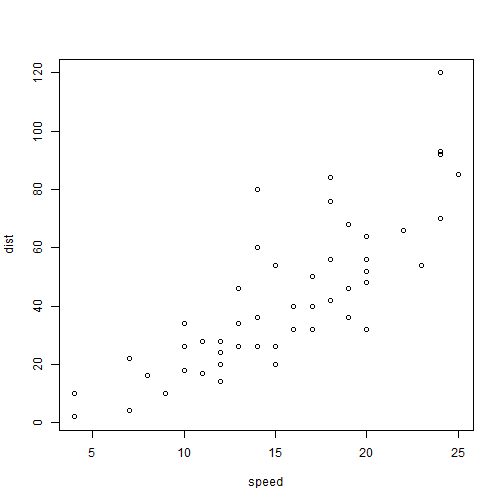
\includegraphics[width=0.7\linewidth,height=0.7\textheight]{Lesson-7-Companion_files/figure-latex/unnamed-chunk-2-1} \end{center}

\begin{Shaded}
\begin{Highlighting}[]
\CommentTok{#Find the two-sided p-value}
\NormalTok{replications_dataframe }\OperatorTok
\StringTok{  }\KeywordTok{summarise}\NormalTok{(}\DataTypeTok{pvalue =}\NormalTok{ (}\KeywordTok{sum}\NormalTok{(trial_stat }\OperatorTok{<=}\StringTok{ }\NormalTok{below) }\OperatorTok{+}\StringTok{ }
\StringTok{              }\KeywordTok{sum}\NormalTok{(trial_stat }\OperatorTok{>=}\StringTok{ }\NormalTok{above)) }\OperatorTok{/}\StringTok{ }\KeywordTok{n}\NormalTok{())}
\end{Highlighting}
\end{Shaded}

\begin{verbatim}
##   pvalue
## 1  0.001
\end{verbatim}

\hypertarget{one-sample-t-test}{%
\subsubsection{One-sample t-test}\label{one-sample-t-test}}

I'm going to first show you a method that will, hopefully, help you
understand calculating the p-value\ldots{} and then I'm going to show
you the easy way. We'll continue with the same example and check our
validity conditions.

\begin{Shaded}
\begin{Highlighting}[]
\CommentTok{#At least 20 observations...}
\KeywordTok{nrow}\NormalTok{(estimates)}
\end{Highlighting}
\end{Shaded}

\begin{verbatim}
## [1] 25
\end{verbatim}

\begin{Shaded}
\begin{Highlighting}[]
\CommentTok{#...and their distribution should not be strongly skewed}
\NormalTok{estimates }\OperatorTok
\StringTok{  }\KeywordTok{ggplot}\NormalTok{(}\KeywordTok{aes}\NormalTok{(}\DataTypeTok{x =}\NormalTok{ Time)) }\OperatorTok{+}
\StringTok{  }\KeywordTok{labs}\NormalTok{(}\DataTypeTok{x =} \StringTok{"Time"}\NormalTok{, }\DataTypeTok{y =} \StringTok{"Count"}\NormalTok{, }\DataTypeTok{title =} \StringTok{"Distribution of Original Sample"}\NormalTok{) }\OperatorTok{+}
\StringTok{  }\KeywordTok{geom_histogram}\NormalTok{()}
\end{Highlighting}
\end{Shaded}

\begin{center}\includegraphics[width=0.7\linewidth,height=0.7\textheight]{Lesson-7-Companion_files/figure-latex/unnamed-chunk-3-1} \end{center}

A question you're going to ask again and again is ``how skewed is
\emph{strongly skewed}'' and I would advise you to go check out my
``Normality Testing'' document on GitHub. In the end, I assess this
distribution is not strongly skewed. Now that we've met our validity
conditions, the central limit theorem (CLT) tells us that our ``trial
means'' will be distributed normally if the population is distributed
normally or approximately normally if the sample size is large enough
(regardless of the population distribution). These normal distributions
will have a mean of \(\mu\) and a standard deviation of
\(\frac{\sigma}{\sqrt{n}}\).

But wait, we don't have our population standard deviation (\(\sigma\))
so what do we do? The best we can do is approximate it using the sample
standard deviation(\(s\)). Note: Even though it is named
\emph{new\_population}, our somewhat artificial \emph{population} is not
truely our broader population.

\begin{Shaded}
\begin{Highlighting}[]
\NormalTok{CLT_sd =}\StringTok{ }\KeywordTok{sd}\NormalTok{(new_population}\OperatorTok{$}\NormalTok{Time) }\OperatorTok{/}\StringTok{ }\KeywordTok{sqrt}\NormalTok{(sample_size)}

\NormalTok{replications_dataframe }\OperatorTok
\StringTok{  }\KeywordTok{ggplot}\NormalTok{(}\KeywordTok{aes}\NormalTok{(}\DataTypeTok{x =}\NormalTok{ trial_stat)) }\OperatorTok{+}
\StringTok{  }\KeywordTok{labs}\NormalTok{(}\DataTypeTok{x =} \StringTok{"Trial Mean"}\NormalTok{, }\DataTypeTok{y =} \StringTok{"Density"}\NormalTok{, }
       \DataTypeTok{title =} \StringTok{"Null Distribution and Normal Distribution"}\NormalTok{) }\OperatorTok{+}
\StringTok{  }\KeywordTok{geom_histogram}\NormalTok{(}\KeywordTok{aes}\NormalTok{(}\DataTypeTok{y =}\NormalTok{ ..density..)) }\OperatorTok{+}
\StringTok{  }\KeywordTok{stat_function}\NormalTok{(}\DataTypeTok{fun =}\NormalTok{ dnorm, }
                \DataTypeTok{args =} \KeywordTok{list}\NormalTok{(}\DataTypeTok{mean =}\NormalTok{ null_mean, }\DataTypeTok{sd =}\NormalTok{ CLT_sd),}
                \DataTypeTok{color =} \StringTok{"red"}\NormalTok{)}
\end{Highlighting}
\end{Shaded}

\begin{center}\includegraphics[width=0.7\linewidth,height=0.7\textheight]{Lesson-7-Companion_files/figure-latex/unnamed-chunk-4-1} \end{center}

You might ask ``but how do we account for the uncertainty introduced by
using the sample standard deviation as opposed to the population
standard deviation?'' That's a great question and it explains why the
\textbf{t}-distribution is used instead of the normal distribution. The
t-distribution has ``fatter tails'' than the normal distribution for a
given sample size and therefore you need have a more extreme sample
statistic in order to reject the null hypothesis at a given significance
level (Type 1 Error/False Alarm).

\begin{Shaded}
\begin{Highlighting}[]
\CommentTok{#Just picking a sample size for demonstration}
\NormalTok{n =}\StringTok{ }\DecValTok{3}

\KeywordTok{ggplot}\NormalTok{(}\KeywordTok{data.frame}\NormalTok{(}\DataTypeTok{x =} \KeywordTok{c}\NormalTok{(}\OperatorTok{-}\DecValTok{5}\NormalTok{,}\DecValTok{5}\NormalTok{)), }\KeywordTok{aes}\NormalTok{(}\DataTypeTok{x =}\NormalTok{ x)) }\OperatorTok{+}
\StringTok{  }\KeywordTok{stat_function}\NormalTok{(}\DataTypeTok{fun =}\NormalTok{ dnorm,}
                \DataTypeTok{color =} \StringTok{"blue"}\NormalTok{) }\OperatorTok{+}
\StringTok{  }\KeywordTok{stat_function}\NormalTok{(}\DataTypeTok{fun =}\NormalTok{ dt,}
                \DataTypeTok{args =} \KeywordTok{list}\NormalTok{(}\DataTypeTok{df =}\NormalTok{ n }\OperatorTok{-}\StringTok{ }\DecValTok{1}\NormalTok{),}
                \DataTypeTok{color =} \StringTok{"red"}\NormalTok{)}
\end{Highlighting}
\end{Shaded}

\begin{center}\includegraphics[width=0.7\linewidth,height=0.7\textheight]{Lesson-7-Companion_files/figure-latex/unnamed-chunk-5-1} \end{center}

Other than the extra area in the tails, the t-distribution functions
exactly like the normal distribution for finding our p-value.

\begin{Shaded}
\begin{Highlighting}[]
\CommentTok{#Back to using the estimates dataframe}
\NormalTok{standard_deviation =}\StringTok{ }\KeywordTok{sd}\NormalTok{(estimates}\OperatorTok{$}\NormalTok{Time)}

\NormalTok{sample_size =}\StringTok{ }\KeywordTok{nrow}\NormalTok{(estimates)}

\NormalTok{sample_t_stat =}\StringTok{ }\NormalTok{(sample_stat }\OperatorTok{-}\StringTok{ }\NormalTok{null_mean) }\OperatorTok{/}\StringTok{ }\NormalTok{(standard_deviation }\OperatorTok{/}\StringTok{ }\KeywordTok{sqrt}\NormalTok{(sample_size))}

\CommentTok{#One of the tails (left for this example)}
\KeywordTok{pt}\NormalTok{(}\OperatorTok{-}\NormalTok{sample_t_stat, }\DataTypeTok{df =}\NormalTok{ sample_size }\OperatorTok{-}\StringTok{ }\DecValTok{1}\NormalTok{)}
\end{Highlighting}
\end{Shaded}

\begin{verbatim}
## [1] 0.0009028877
\end{verbatim}

\begin{Shaded}
\begin{Highlighting}[]
\CommentTok{#The other tail (right for this example)}
\DecValTok{1} \OperatorTok{-}\StringTok{ }\KeywordTok{pt}\NormalTok{(sample_t_stat, }\DataTypeTok{df =}\NormalTok{ sample_size }\OperatorTok{-}\StringTok{ }\DecValTok{1}\NormalTok{)}
\end{Highlighting}
\end{Shaded}

\begin{verbatim}
## [1] 0.0009028877
\end{verbatim}

\begin{Shaded}
\begin{Highlighting}[]
\CommentTok{#Both tails together}
\DecValTok{2} \OperatorTok{*}\StringTok{ }\NormalTok{(}\DecValTok{1} \OperatorTok{-}\StringTok{ }\KeywordTok{pt}\NormalTok{(}\KeywordTok{abs}\NormalTok{(sample_t_stat), }\DataTypeTok{df =}\NormalTok{ sample_size }\OperatorTok{-}\StringTok{ }\DecValTok{1}\NormalTok{))}
\end{Highlighting}
\end{Shaded}

\begin{verbatim}
## [1] 0.001805775
\end{verbatim}

The first step here was calculating the t-statistic for our original
sample. It might be hard to remember that original sample at this point
so maybe scroll up to remind yourself. We can then use the \textbf{pt()}
function to find the area under the t-distribution curve. It's like
\textbf{pnorm()} but for the t-distribution instead. In essence we are
looking for the red area in the figure below. Clearly, I've zoomed in
here so you can see the actual area.

\begin{Shaded}
\begin{Highlighting}[]
\KeywordTok{ggplot}\NormalTok{(}\KeywordTok{data.frame}\NormalTok{(}\DataTypeTok{x =} \KeywordTok{c}\NormalTok{(}\OperatorTok{-}\DecValTok{5}\NormalTok{, }\DecValTok{5}\NormalTok{)), }\KeywordTok{aes}\NormalTok{(}\DataTypeTok{x =}\NormalTok{ x)) }\OperatorTok{+}
\StringTok{    }\KeywordTok{stat_function}\NormalTok{(}\DataTypeTok{fun =}\NormalTok{ dt, }
                \DataTypeTok{args =} \KeywordTok{list}\NormalTok{(}\DataTypeTok{df =}\NormalTok{ sample_size }\OperatorTok{-}\StringTok{ }\DecValTok{1}\NormalTok{)) }\OperatorTok{+}
\StringTok{  }\KeywordTok{geom_vline}\NormalTok{(}\DataTypeTok{xintercept =}\NormalTok{ sample_t_stat, }\DataTypeTok{color =} \StringTok{"red"}\NormalTok{) }\OperatorTok{+}
\StringTok{  }\KeywordTok{geom_vline}\NormalTok{(}\DataTypeTok{xintercept =} \OperatorTok{-}\NormalTok{sample_t_stat, }\DataTypeTok{color =} \StringTok{"red"}\NormalTok{) }\OperatorTok{+}
\StringTok{  }\KeywordTok{stat_function}\NormalTok{(}\DataTypeTok{fun =}\NormalTok{ dt, }
                \DataTypeTok{args =} \KeywordTok{list}\NormalTok{(}\DataTypeTok{df =}\NormalTok{ sample_size }\OperatorTok{-}\StringTok{ }\DecValTok{1}\NormalTok{),}
                \DataTypeTok{xlim =} \KeywordTok{c}\NormalTok{(}\OperatorTok{-}\DecValTok{5}\NormalTok{, }\OperatorTok{-}\NormalTok{sample_t_stat),}
                \DataTypeTok{geom =} \StringTok{"area"}\NormalTok{, }\DataTypeTok{fill =} \StringTok{"red"}\NormalTok{) }\OperatorTok{+}
\StringTok{    }\KeywordTok{stat_function}\NormalTok{(}\DataTypeTok{fun =}\NormalTok{ dt, }
                \DataTypeTok{args =} \KeywordTok{list}\NormalTok{(}\DataTypeTok{df =}\NormalTok{ sample_size }\OperatorTok{-}\StringTok{ }\DecValTok{1}\NormalTok{),}
                \DataTypeTok{xlim =} \KeywordTok{c}\NormalTok{(sample_t_stat, }\DecValTok{5}\NormalTok{),}
                \DataTypeTok{geom =} \StringTok{"area"}\NormalTok{, }\DataTypeTok{fill =} \StringTok{"red"}\NormalTok{) }\OperatorTok{+}
\StringTok{  }\KeywordTok{labs}\NormalTok{(}\DataTypeTok{x =} \StringTok{""}\NormalTok{, }\DataTypeTok{y =} \StringTok{""}\NormalTok{) }\OperatorTok{+}\StringTok{ }\KeywordTok{theme_classic}\NormalTok{() }\OperatorTok{+}\StringTok{ }\KeywordTok{ylim}\NormalTok{(}\KeywordTok{c}\NormalTok{(}\DecValTok{0}\NormalTok{, }\FloatTok{0.01}\NormalTok{))}
\end{Highlighting}
\end{Shaded}

\begin{center}\includegraphics[width=0.7\linewidth,height=0.7\textheight]{Lesson-7-Companion_files/figure-latex/unnamed-chunk-7-1} \end{center}

While I think it's important for you to know how to use the
\textbf{pt()} function because it promotes a deeper understanding,
\emph{R} has another function that will allow you to quickly calculate
the p-value.

\begin{Shaded}
\begin{Highlighting}[]
\KeywordTok{t.test}\NormalTok{(estimates, }\DataTypeTok{mu =}\NormalTok{ null_mean, }\DataTypeTok{alternative =} \StringTok{"two.sided"}\NormalTok{)}
\end{Highlighting}
\end{Shaded}

\begin{verbatim}
## 
##  One Sample t-test
## 
## data:  estimates
## t = 3.5081, df = 24, p-value = 0.001806
## alternative hypothesis: true mean is not equal to 10
## 95 percent confidence interval:
##  11.56437 16.03563
## sample estimates:
## mean of x 
##      13.8
\end{verbatim}

Yes, that was \textbf{a lot} less code. Spend some time playing around
with the parameters of \textbf{t.test()} so you become familiar with
what each does and how to apply this function to different types of
problems.

\end{document}
